\documentclass[tikz,border=2pt]{standalone}
\usetikzlibrary{arrows.meta,positioning,fit,calc,shapes.geometric,decorations.pathmorphing}
\definecolor{blueMain}{HTML}{0B4E94}
\definecolor{blueSoft}{HTML}{EAF2FA}
\definecolor{tealMain}{HTML}{3B9AA3}
\definecolor{greenSoft}{HTML}{DDF3DE}
\definecolor{redMain}{HTML}{B64342}
\definecolor{redSoft}{HTML}{F6CFCB}
\definecolor{goldMain}{HTML}{D99A21}
\definecolor{goldSoft}{HTML}{FFF2CC}
\definecolor{violetMain}{HTML}{6B3FB4}
\definecolor{greyText}{HTML}{222222}
\definecolor{greyLine}{HTML}{9A9A9A}
\definecolor{panel}{HTML}{F7F7F7}
\tikzset{
  blk/.style={draw=#1, rounded corners=2pt, thick, align=center, fill=white,
    inner sep=2.4pt, font=\sffamily\scriptsize},
  dashedblk/.style={draw=#1, dashed, rounded corners=2pt, thick, align=center,
    fill=white, inner sep=2.4pt, font=\sffamily\scriptsize},
  arr/.style={-{Stealth[length=2mm]}, thick},
  num/.style={circle, draw=blueMain, text=blueMain, fill=white, inner sep=0.45pt,
    minimum size=0.23cm, font=\sffamily\tiny\bfseries},
  tinytext/.style={font=\sffamily\tiny, align=center},
  dev/.style={circle, draw=greyText, fill=white, minimum size=4pt, inner sep=0pt}
}
\newcommand{\Step}[3]{\node[num] at (#1,#2) {#3};}
\begin{document}
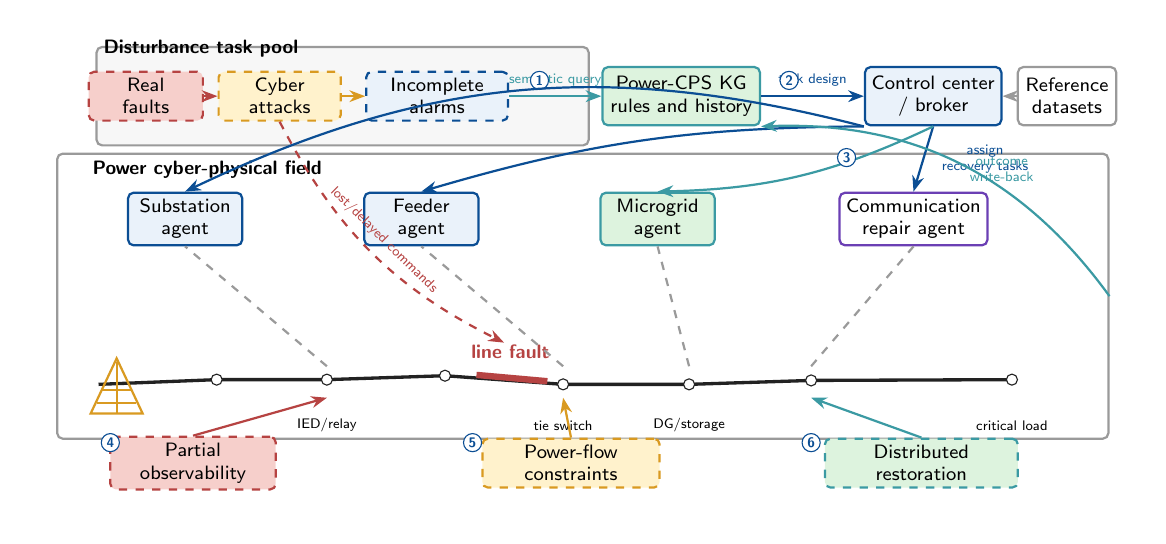
\begin{tikzpicture}[x=1cm,y=1cm,font=\sffamily\scriptsize]
  \path[use as bounding box] (0.05,0.05) rectangle (14.15,6.25);

  % Top task and knowledge pool, following the template-style FL task pool.
  \node[blk=greyLine, fill=panel, minimum width=6.25cm, minimum height=1.25cm] (pool) at (4.05,5.38) {};
  \node[font=\sffamily\scriptsize\bfseries] at (2.25,5.98) {Disturbance task pool};
  \node[dashedblk=redMain, fill=redSoft, minimum width=1.45cm, minimum height=0.62cm] (real) at (1.55,5.38) {Real\\faults};
  \node[dashedblk=goldMain, fill=goldSoft, minimum width=1.55cm, minimum height=0.62cm] (cyber) at (3.25,5.38) {Cyber\\attacks};
  \node[dashedblk=blueMain, fill=blueSoft, minimum width=1.80cm, minimum height=0.62cm] (uncertain) at (5.25,5.38) {Incomplete\\alarms};
  \node[blk=tealMain, fill=greenSoft, minimum width=2.00cm, minimum height=0.74cm] (kg) at (8.35,5.38) {Power-CPS KG\\rules and history};
  \node[blk=blueMain, fill=blueSoft, minimum width=1.70cm, minimum height=0.74cm] (broker) at (11.55,5.38) {Control center\\/ broker};
  \node[blk=greyLine, fill=white, minimum width=1.25cm, minimum height=0.74cm] (ref) at (13.25,5.38) {Reference\\datasets};

  \draw[arr, redMain] (real.east) -- (cyber.west);
  \draw[arr, goldMain] (cyber.east) -- (uncertain.west);
  \draw[arr, tealMain] (uncertain.east) -- node[above,tinytext] {semantic query} (kg.west);
  \draw[arr, blueMain] (kg.east) -- node[above,tinytext] {task design} (broker.west);
  \draw[arr, greyLine] (ref.west) -- (broker.east);
  \Step{6.55}{5.58}{1}
  \Step{9.72}{5.58}{2}

  % Physical-cyber field.
  \node[blk=greyLine, fill=white, minimum width=13.35cm, minimum height=3.62cm] (field) at (7.10,2.84) {};
  \node[anchor=west, font=\sffamily\scriptsize\bfseries] at (0.75,4.45) {Power cyber-physical field};

  \node[blk=blueMain, fill=blueSoft, minimum width=1.45cm] (sub) at (2.05,3.82) {Substation\\agent};
  \node[blk=blueMain, fill=blueSoft, minimum width=1.45cm] (feed) at (5.05,3.82) {Feeder\\agent};
  \node[blk=tealMain, fill=greenSoft, minimum width=1.45cm] (mg) at (8.05,3.82) {Microgrid\\agent};
  \node[blk=violetMain, fill=white, minimum width=1.75cm] (comm) at (11.30,3.82) {Communication\\repair agent};

  \draw[arr, blueMain] (broker.south) -- node[right,tinytext, xshift=3pt] {assign\\recovery tasks} (comm.north);
  \draw[arr, blueMain] (broker.south west) to[bend right=20] (sub.north);
  \draw[arr, blueMain] (broker.south west) to[bend right=8] (feed.north);
  \draw[arr, tealMain] (broker.south) to[bend left=12] (mg.north);
  \Step{10.45}{4.60}{3}

  % Physical feeder line.
  \draw[very thick, greyText] (0.95,1.72) -- (2.45,1.78) -- (3.85,1.78) -- (5.35,1.83) -- (6.85,1.72) -- (8.45,1.72) -- (10.00,1.77) -- (12.55,1.78);
  \foreach \x/\y in {2.45/1.78,3.85/1.78,5.35/1.83,6.85/1.72,8.45/1.72,10.00/1.77,12.55/1.78}
    \node[dev] at (\x,\y) {};
  \draw[goldMain, thick] (0.85,1.35) -- (1.18,2.05) -- (1.51,1.35) -- cycle;
  \draw[goldMain, thick] (1.18,2.00) -- (1.18,1.36);
  \draw[goldMain, thick] (1.00,1.65) -- (1.36,1.65);
  \draw[goldMain, thick] (0.93,1.48) -- (1.43,1.48);
  \draw[redMain, line width=2.3pt] (5.75,1.84) -- (6.65,1.76);
  \node[text=redMain, font=\sffamily\scriptsize\bfseries] at (6.18,2.13) {line fault};
  \node[tinytext] at (3.85,1.20) {IED/relay};
  \node[tinytext] at (6.85,1.20) {tie switch};
  \node[tinytext] at (8.45,1.20) {DG/storage};
  \node[tinytext] at (12.55,1.20) {critical load};

  % Needs and checks, template-like lower boxes.
  \node[dashedblk=redMain, fill=redSoft, minimum width=2.10cm] (obs) at (2.15,0.72) {Partial\\observability};
  \node[dashedblk=goldMain, fill=goldSoft, minimum width=2.25cm] (phy) at (6.95,0.72) {Power-flow\\constraints};
  \node[dashedblk=tealMain, fill=greenSoft, minimum width=2.45cm] (dist) at (11.40,0.72) {Distributed\\restoration};
  \draw[arr, redMain] (obs.north) -- (3.85,1.55);
  \draw[arr, goldMain] (phy.north) -- (6.85,1.55);
  \draw[arr, tealMain] (dist.north) -- (10.00,1.55);
  \Step{1.10}{0.98}{4}
  \Step{5.70}{0.98}{5}
  \Step{10.00}{0.98}{6}

  % Cross-layer evidence and command links.
  \foreach \x/\agt in {3.85/sub,6.85/feed,8.45/mg,10.00/comm}
    \draw[dashed, greyLine, thick] (\x,1.95) -- (\agt.south);
  \draw[arr, redMain, dashed] (cyber.south) to[bend right=18] node[tinytext,above,sloped] {lost/delayed commands} (6.10,2.25);
  \draw[arr, tealMain] (field.east) to[bend right=28] (kg.south east);
  \node[tinytext, text=tealMain] at (12.42,4.45) {outcome\\write-back};
\end{tikzpicture}
\end{document}
